\chapter{Evaluation}
\label{chap:evaluation}

The presented map-merging algorithm (chapter~\ref{chap:mergingalgorithm}) has been evaluated on number of demanding robotics datasets. The datasets include data captured by small aerial vehicles (sections~\ref{sec:euroc-dataset}, \ref{sec:aau-dataset}) as well as ground-based robots. The datasets include both widely used benchmark datasets in robotics research as well as data recorded by the author.

Sensors used include stereo rig cameras, active \gls{RGB-D} cameras and laser range finders? This variety of sensors and robots covers many typical multi-robot deployments. All datasets has been captured under real-word conditions, none of them uses simulated data.

The evaluation focuses on properties of the presented pair-wise transformation estimation algorithm for pointclouds (section~\ref{sec:estimate-pair-wise}), which is the core algorithm of the implemented map-merging \gls{ROS} node (section~\ref{sec:ros-package}). Accuracy of the estimation algorithm is critical for the overall map-merging process.

\section{The EuRoC micro aerial vehicle datasets}
\label{sec:euroc-dataset}

The publicly available dataset introduced by~\citet{Burri2016} was collected on-board a micro aerial vehicle (figure~\ref{fig:euroc_platform}) equipped with stereo camera rig and \gls{IMU}. Calibration data for the cameras and ground-truth data are provided with the dataset. This dataset has been used extensively by researches for evaluation of the visual \gls{SLAM} algorithms and visual odometry approaches.

\begin{figure}
    \centering
    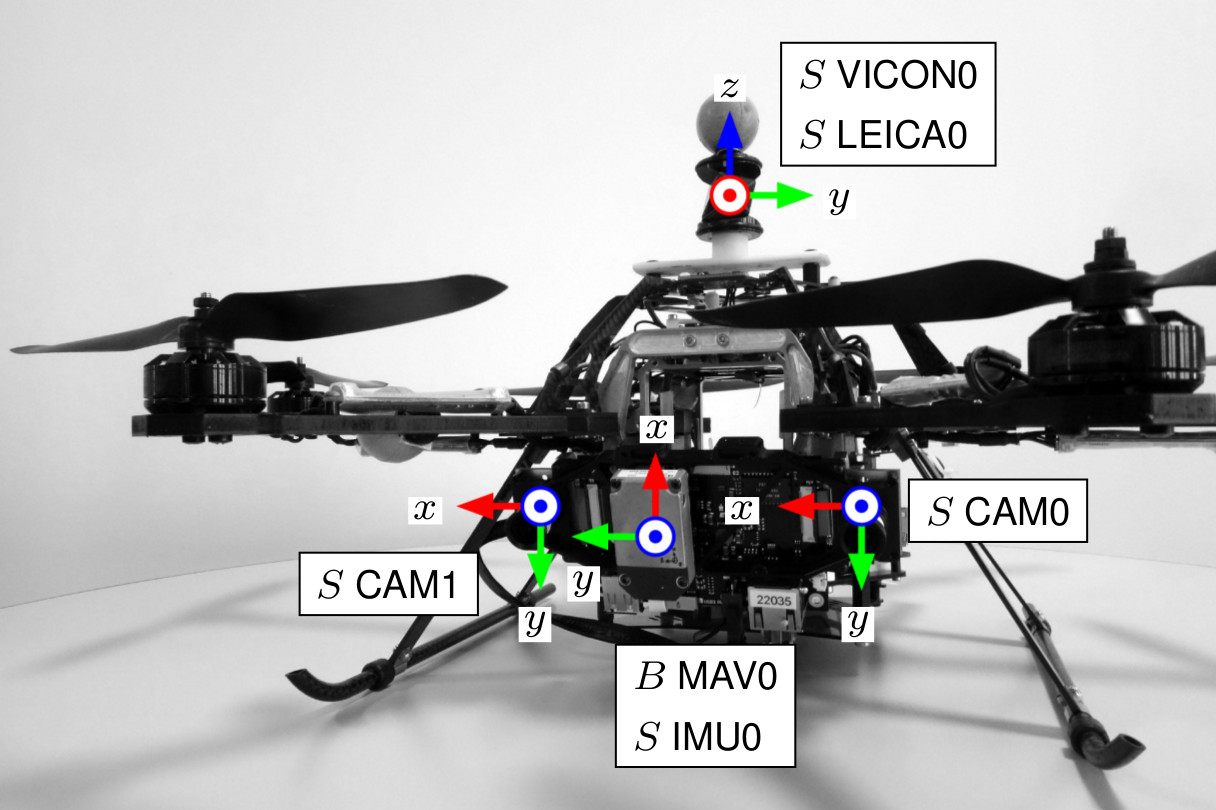
\includegraphics[width=\textwidth]{../img/euroc_platform.jpg}
    \caption[A micro aerial vehicle]{An Asctec Firefly hex-rotor micro aerial vehicle used for collecting the EuRoC micro aerial vehicle datasets. The picture shows reference frames of the sensors -- the stereo cameras and \gls{IMU}.}
    \label{fig:euroc_platform}
\end{figure}

\subsection{Dataset description}

The cameras produce a WVGA monochrome (greyscale) images at $20$ frames per second. Cameras have a global shutter. The automatic exposure control is independent for both cameras. According to the published errata~\citep{Burri2016}, this ``resulted in different shutter times and in turn in different image brightnesses, rendering stereo matching and feature tracking more challenging''.

The dataset contains $11$ mapping sessions in $3$ different environments (``Machine Hall'', ``Vicon Room 1'', ``Vicon Room 2''). Each mapping session is available in a single \gls{ROS} bag file. First $5$ sessions were captured in ETH machine hall (figure~\ref{fig:eth-machine-hall}), a fairly large industrial environment featuring piping, reservoirs and many different types of surfaces. Second and third batch of datasets were captured in a smaller furnished rectangular room. For the second and the third batch the furnishing was different.

\begin{figure}
    \centering
    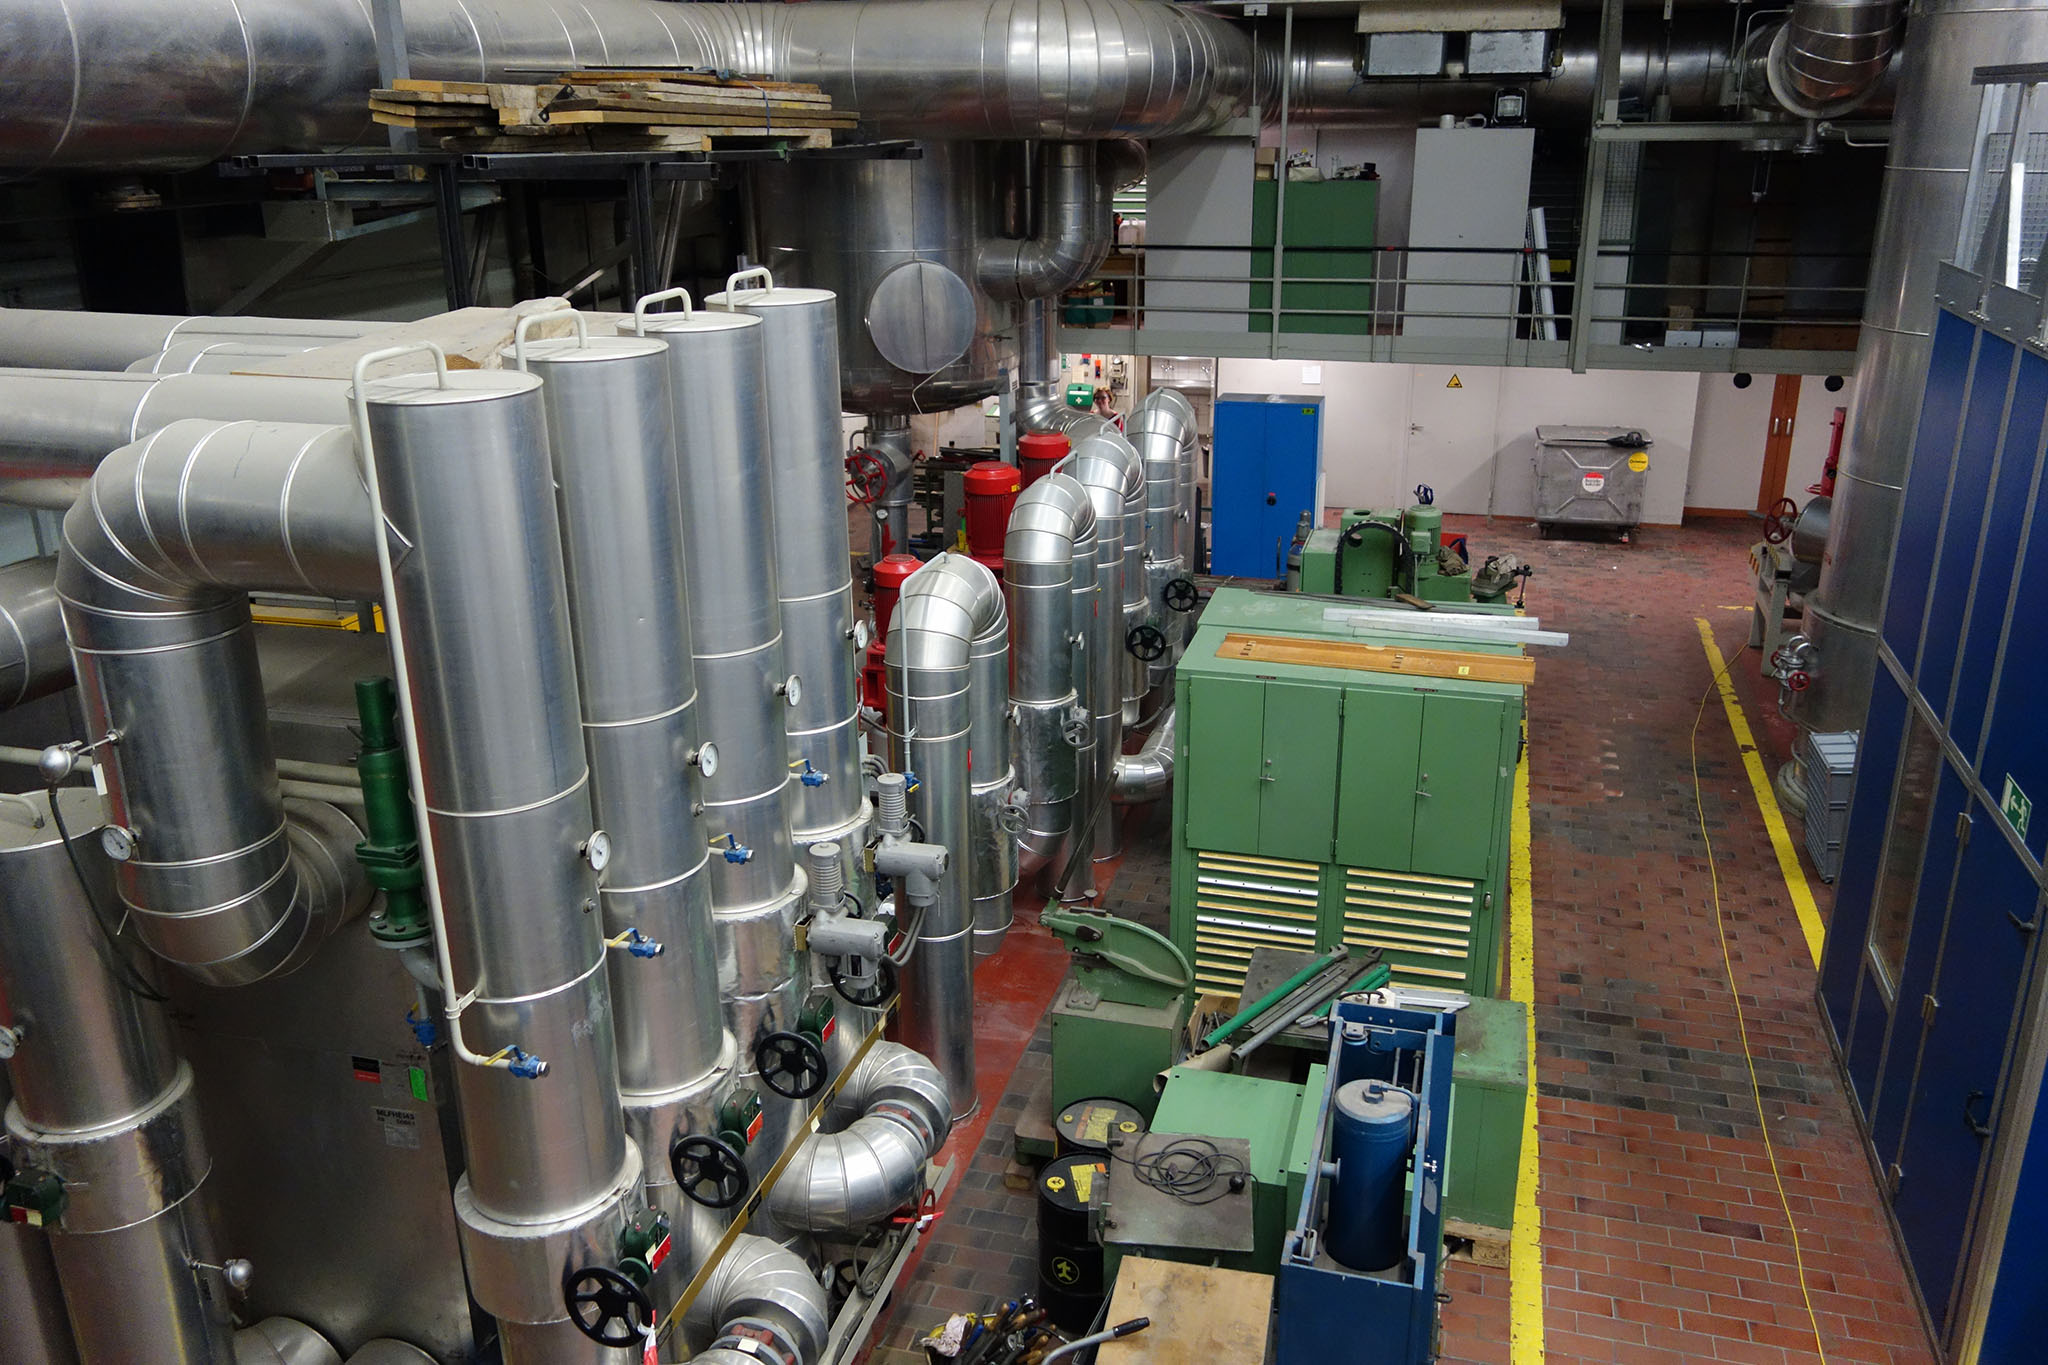
\includegraphics[width=\textwidth]{../img/eth_machine_room.jpg}
    \caption[ETH Machine hall]{ETH Machine hall industrial environment where $5$ mapping sessions of EuRoC dataset were captured. The image is courtesy of the authors~\citep{Burri2016}.}
    \label{fig:eth-machine-hall}
\end{figure}

\subsection{Maps generation}
\label{sec:euroc-generating-maps}

The dataset is intended for evaluating \gls{SLAM} algorithms, for our purposes it was necessary to process the data with a \gls{SLAM} algorithm to create a pointcloud maps.

First, I have used the provided calibration sequence and I have created a calibration data for \gls{ROS} using the \texttt{camera\_calibration} tool available with \gls{ROS}.

Second, for each environment I created a pair of maps using the $01$ and $02$ mapping sessions from the datasets, which were used further for the evaluation of the map-merging (figures~\ref{fig:euroc_mh_02}, \ref{fig:v1-greyscale}, \ref{fig:euroc_v2_02}). I used a RTAB-Map \gls{SLAM}, developed by~\citet{labbe2014online}, to create the maps. The odometry for mapping was provided from stereo camera data, using a visual odometry approach, the available \gls{IMU} data were not used. For the $01$ sessions I have used a native visual odometry approach of RTAB-Map. For the $02$ sessions I have used visual odometry approach of {ORB-SLAM2}, introduced by~\citet{mur2017orb}, because the data exhibit more dynamic motions, which lead to frequent loss on visual odometry using the first approach. {ORB-SLAM2} visual odometry exhibited better robustness for this data. In both cases loop-closure approach of~\citet{labbe2014online} has been used.

The maps has been voxelised to the resolution of $0.05$ meter per voxel, which yields suitable map sizes for map exchange in a multi-robot system.

Using a different \gls{SLAM} pipelines for each of the maps contributed to introducing different mapping errors and artefacts, which makes map-merging of such maps more difficult.

\begin{figure}
    \centering
    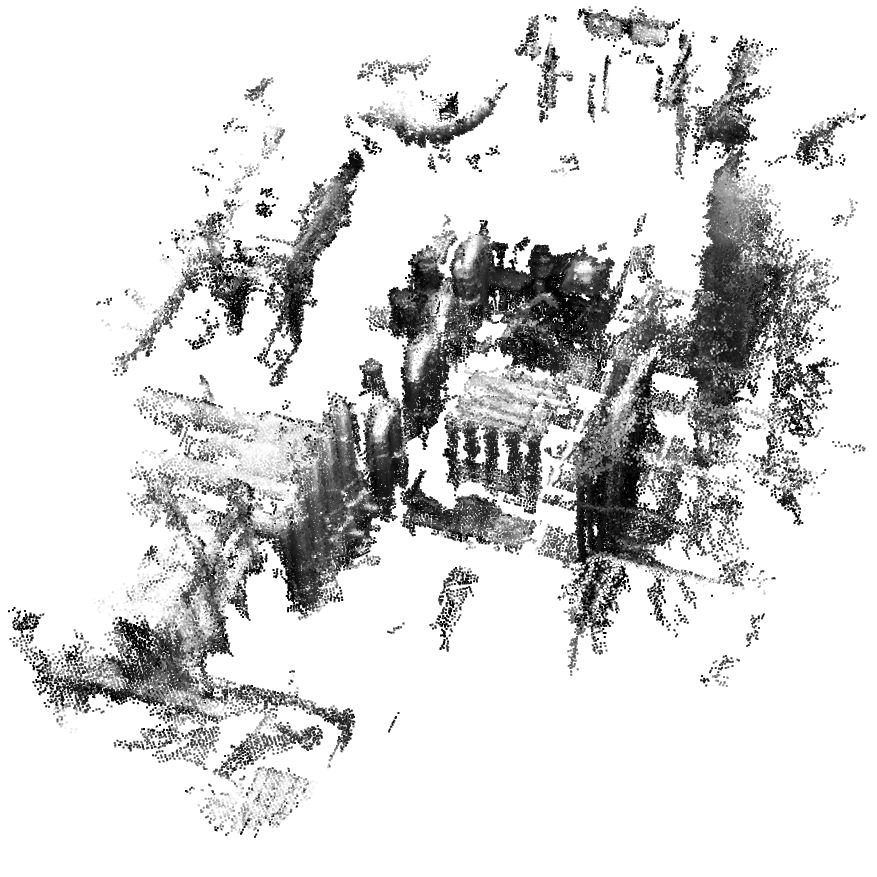
\includegraphics[width=\textwidth]{../img/euroc_mh_02.png}
    \caption[Machine hall pointcloud map]{ETH Machine hall pointcloud map. The map was produced from ``Machine Hall 02'' dataset using an {ORB-SLAM2} visual odometry~\citep{mur2017orb} and RTAB-Map loop-closure approach~\citep{labbe2014online}.}
    \label{fig:euroc_mh_02}
\end{figure}

\begin{figure}
    \centering
    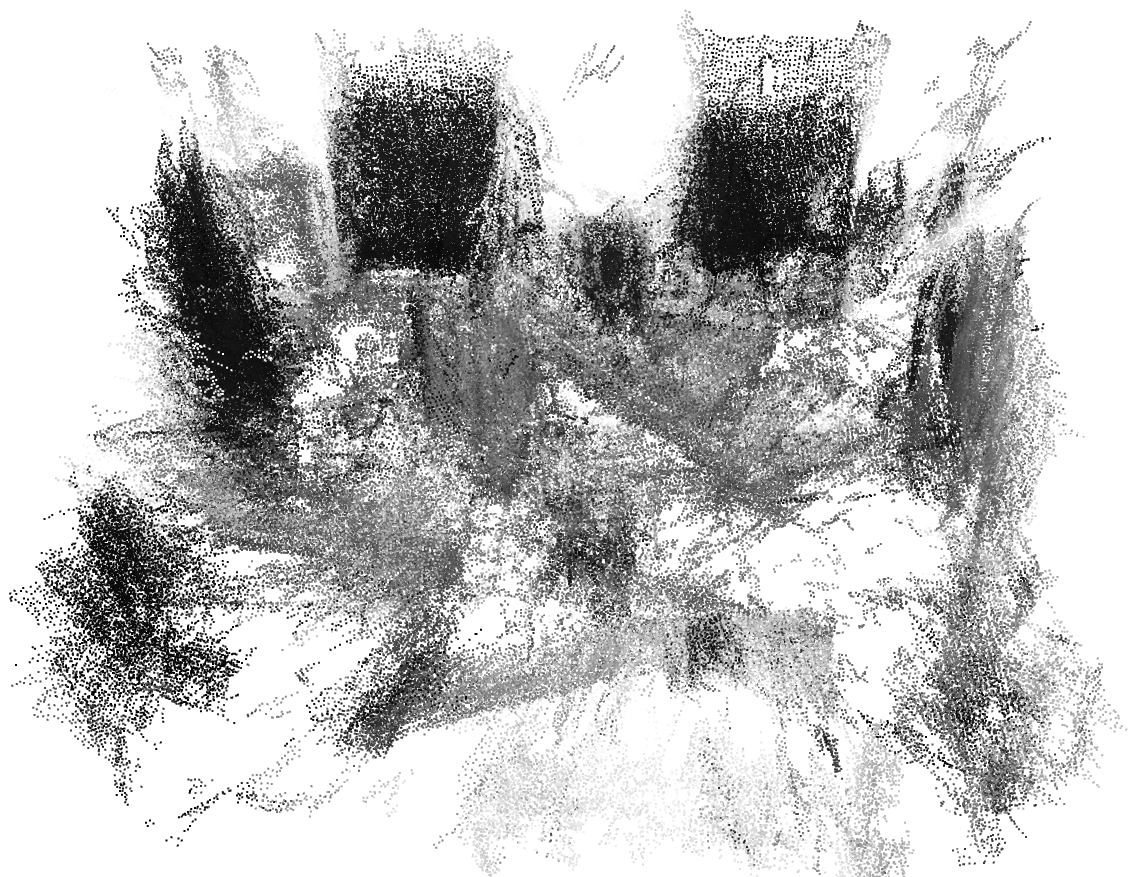
\includegraphics[width=\textwidth]{../img/euroc_v2_02.png}
    \caption[Pointcloud map of a small room]{A pointcloud map of a small room. The map was produced from ``Vicon Room 2 02'' dataset using an {ORB-SLAM2} visual odometry~\citep{mur2017orb} and RTAB-Map loop-closure approach~\citep{labbe2014online}.}
    \label{fig:euroc_v2_02}
\end{figure}

\section{AAU dataset}
\label{sec:aau-dataset}

The dataset recorded at \acrfull{AAU} on-board a micro aerial vehicle in an outdoor forest environment. The vehicle was equipped with a stereo camera rig and \gls{IMU}. The cameras produce greyscale images.

This dataset contains two mapping sessions. The environment consists or medium-sized trees, the ground is covered with leaves. The lighting conditions are challenging as there are areas of direct sunlight as well as areas in the shade. The lighting conditions are similar in the both sessions, as the sessions were captured in the similar time of day. This setup causes difficult conditions for stereo matching and pose estimation, introducing mapping errors into the maps, which in turn make the map-merging a challenging task.

Maps (figures~\ref{fig:aau_top}, \ref{fig:aau_lateral}) were generated in the similar manner as described in section~\ref{sec:euroc-generating-maps}. Mapping has been done with RTAB-Map \gls{SLAM}~\citep{labbe2014online} using a its native visual odometry approach.

% todo atribution

\begin{figure}
    \centering
    \begin{subfigure}[b]{0.82\textwidth}
        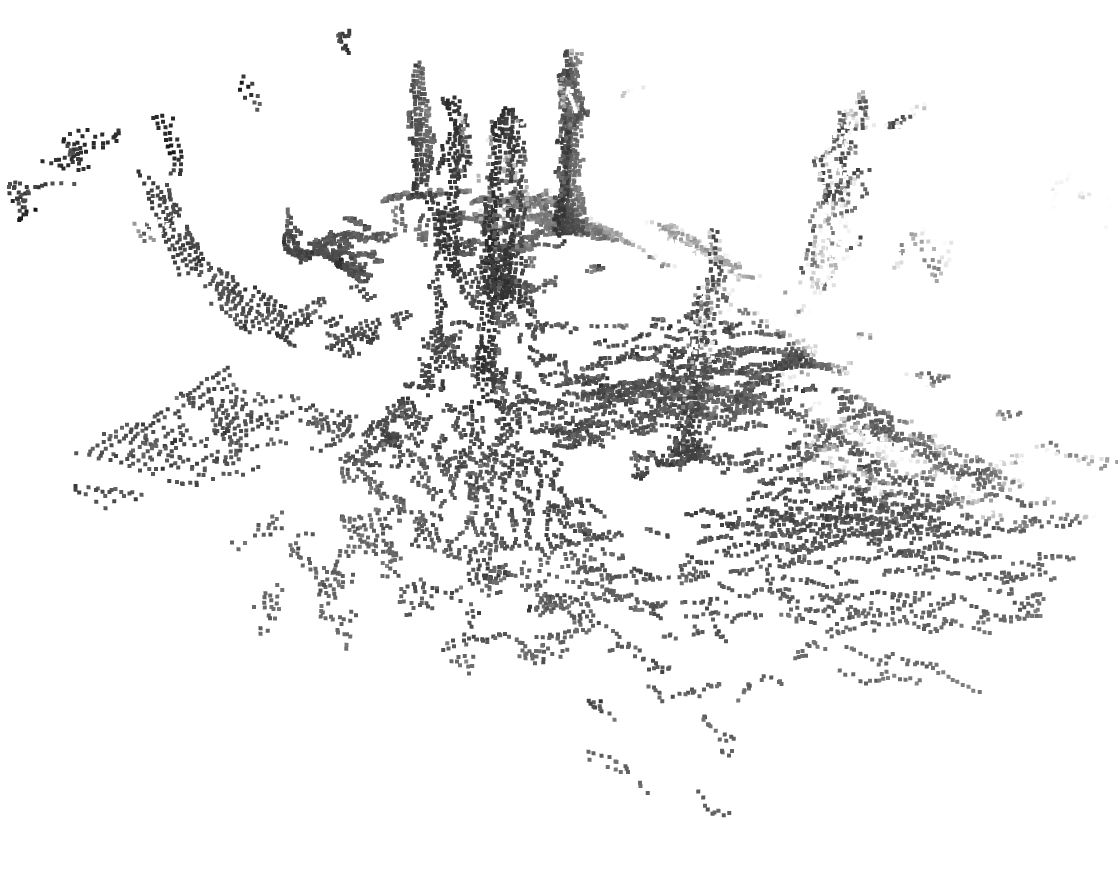
\includegraphics[width=\textwidth]{../img/aau_fc_dnav5_top.png}
        \caption{``\gls{AAU} forest 1'' map}
    \end{subfigure}
    % ~
    \begin{subfigure}[b]{0.82\textwidth}
        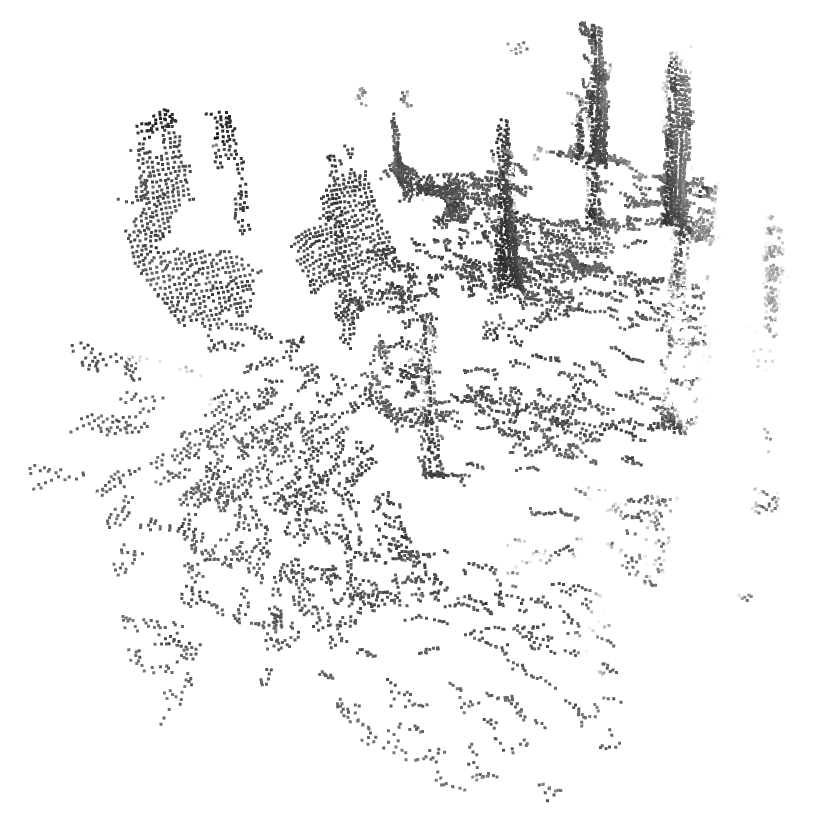
\includegraphics[width=\textwidth]{../img/aau_fc_dnav6_top.png}
        \caption{``\gls{AAU} forest 2'' map}
    \end{subfigure}
    \caption[Forest pointcloud maps -- top view]{Top view of the two pointcloud maps from \gls{AAU} outdoor forest dataset. Notice the stripe of direct sunlight on the ground causing difficult conditions for stereo matching.}
    \label{fig:aau_top}
\end{figure}

\begin{figure}
    \centering
    \begin{subfigure}[b]{\textwidth}
        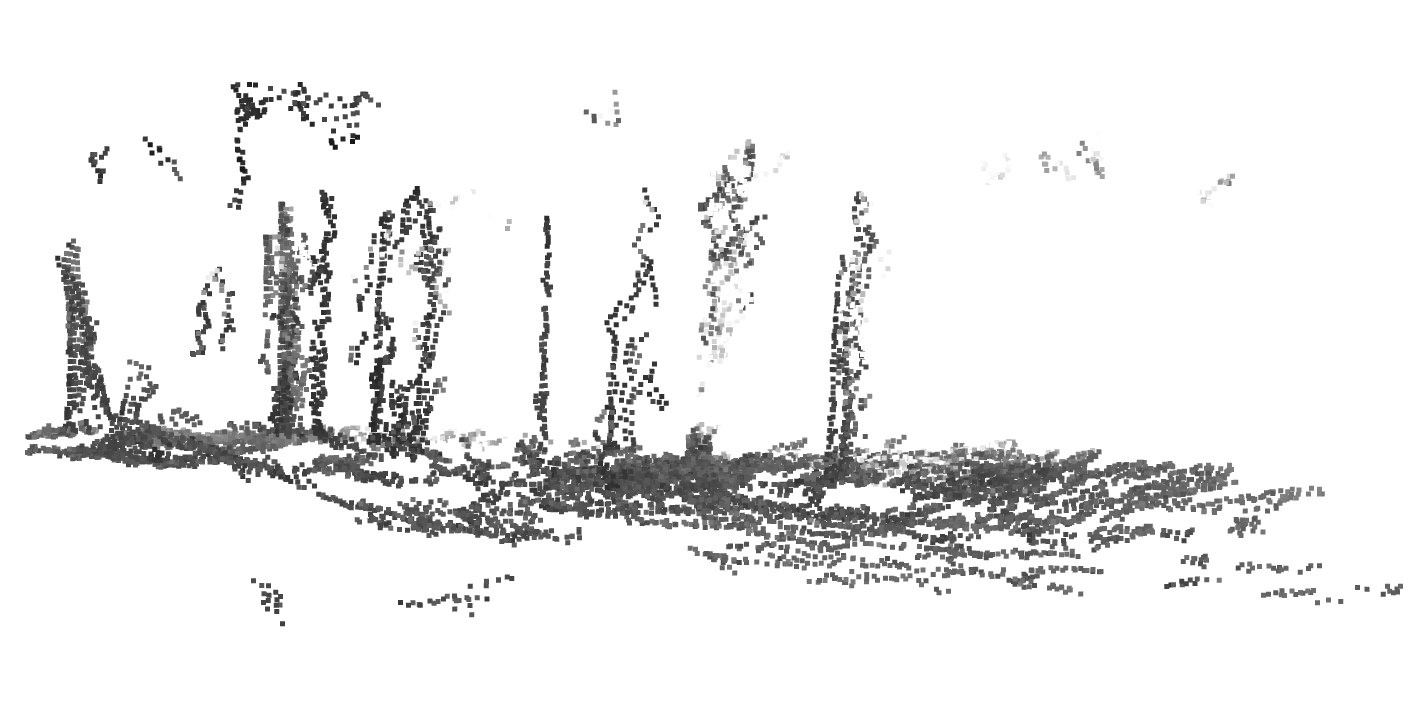
\includegraphics[width=\textwidth]{../img/aau_fc_dnav5_lateral.png}
        \caption{``\gls{AAU} forest 1'' map}
    \end{subfigure}
    % ~
    \begin{subfigure}[b]{\textwidth}
        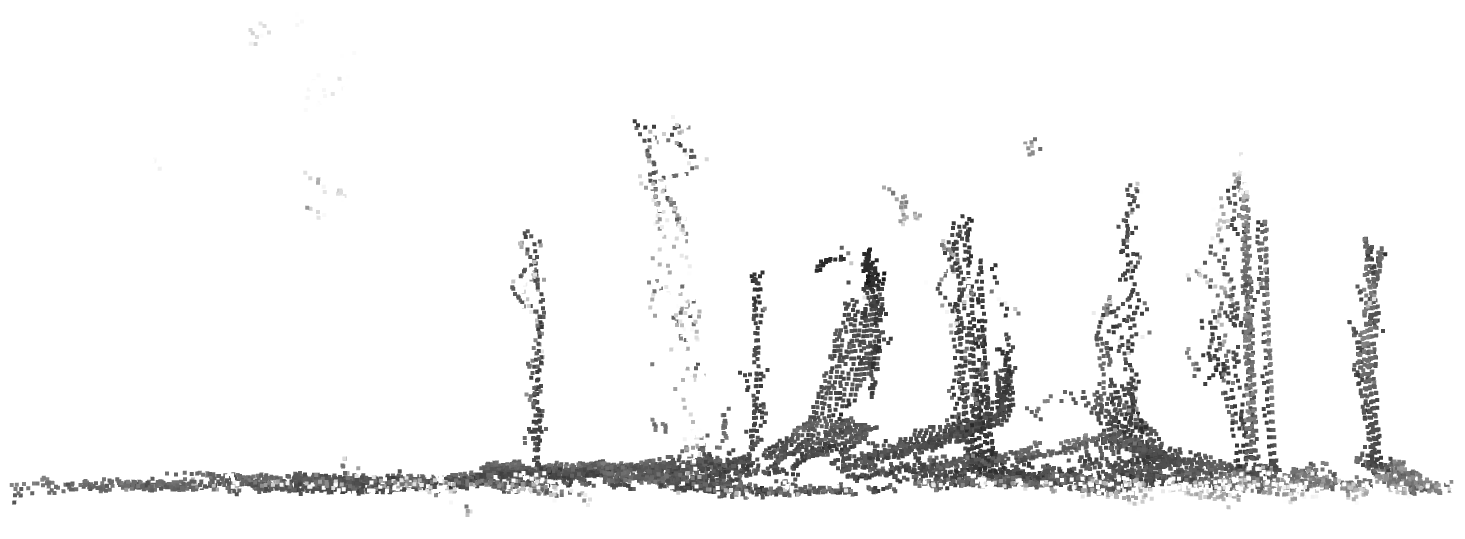
\includegraphics[width=\textwidth]{../img/aau_fc_dnav6_lateral.png}
        \caption{``\gls{AAU} forest 2'' map}
    \end{subfigure}
    \caption[Forest pointcloud maps -- lateral view]{Lateral view of the two pointcloud maps from \gls{AAU} outdoor forest dataset. In both maps there is a non-flat terrain and number of outliers caused by branches and difficult mapping conditions.}
    \label{fig:aau_lateral}
\end{figure}

\section{MFF dataset}
\label{sec:mff-dataset}

\section{Accuracy}

For both the aerial datasets the map-merging is able to correctly merge the maps. The euclidean error scores, according to section~\ref{sec:transform-evaluation}, are small across the datasets (figure~\ref{fig:plot:euc_dist}). There are larger errors for the ``AAU forest'' and ``Machine Hall'' datasets caused by the outliers and mapping errors in those datasets, as those datasets has been recorded in tough conditions. Considering the artefacts in the datasets the alignment almost perfect and would allow precise coordination of the robots.

\begin{figure}
  \centering
  % GNUPLOT: LaTeX picture with Postscript
\begingroup
  \makeatletter
  \providecommand\color[2][]{%
    \GenericError{(gnuplot) \space\space\space\@spaces}{%
      Package color not loaded in conjunction with
      terminal option `colourtext'%
    }{See the gnuplot documentation for explanation.%
    }{Either use 'blacktext' in gnuplot or load the package
      color.sty in LaTeX.}%
    \renewcommand\color[2][]{}%
  }%
  \providecommand\includegraphics[2][]{%
    \GenericError{(gnuplot) \space\space\space\@spaces}{%
      Package graphicx or graphics not loaded%
    }{See the gnuplot documentation for explanation.%
    }{The gnuplot epslatex terminal needs graphicx.sty or graphics.sty.}%
    \renewcommand\includegraphics[2][]{}%
  }%
  \providecommand\rotatebox[2]{#2}%
  \@ifundefined{ifGPcolor}{%
    \newif\ifGPcolor
    \GPcolortrue
  }{}%
  \@ifundefined{ifGPblacktext}{%
    \newif\ifGPblacktext
    \GPblacktextfalse
  }{}%
  % define a \g@addto@macro without @ in the name:
  \let\gplgaddtomacro\g@addto@macro
  % define empty templates for all commands taking text:
  \gdef\gplbacktext{}%
  \gdef\gplfronttext{}%
  \makeatother
  \ifGPblacktext
    % no textcolor at all
    \def\colorrgb#1{}%
    \def\colorgray#1{}%
  \else
    % gray or color?
    \ifGPcolor
      \def\colorrgb#1{\color[rgb]{#1}}%
      \def\colorgray#1{\color[gray]{#1}}%
      \expandafter\def\csname LTw\endcsname{\color{white}}%
      \expandafter\def\csname LTb\endcsname{\color{black}}%
      \expandafter\def\csname LTa\endcsname{\color{black}}%
      \expandafter\def\csname LT0\endcsname{\color[rgb]{1,0,0}}%
      \expandafter\def\csname LT1\endcsname{\color[rgb]{0,1,0}}%
      \expandafter\def\csname LT2\endcsname{\color[rgb]{0,0,1}}%
      \expandafter\def\csname LT3\endcsname{\color[rgb]{1,0,1}}%
      \expandafter\def\csname LT4\endcsname{\color[rgb]{0,1,1}}%
      \expandafter\def\csname LT5\endcsname{\color[rgb]{1,1,0}}%
      \expandafter\def\csname LT6\endcsname{\color[rgb]{0,0,0}}%
      \expandafter\def\csname LT7\endcsname{\color[rgb]{1,0.3,0}}%
      \expandafter\def\csname LT8\endcsname{\color[rgb]{0.5,0.5,0.5}}%
    \else
      % gray
      \def\colorrgb#1{\color{black}}%
      \def\colorgray#1{\color[gray]{#1}}%
      \expandafter\def\csname LTw\endcsname{\color{white}}%
      \expandafter\def\csname LTb\endcsname{\color{black}}%
      \expandafter\def\csname LTa\endcsname{\color{black}}%
      \expandafter\def\csname LT0\endcsname{\color{black}}%
      \expandafter\def\csname LT1\endcsname{\color{black}}%
      \expandafter\def\csname LT2\endcsname{\color{black}}%
      \expandafter\def\csname LT3\endcsname{\color{black}}%
      \expandafter\def\csname LT4\endcsname{\color{black}}%
      \expandafter\def\csname LT5\endcsname{\color{black}}%
      \expandafter\def\csname LT6\endcsname{\color{black}}%
      \expandafter\def\csname LT7\endcsname{\color{black}}%
      \expandafter\def\csname LT8\endcsname{\color{black}}%
    \fi
  \fi
    \setlength{\unitlength}{0.0500bp}%
    \ifx\gptboxheight\undefined%
      \newlength{\gptboxheight}%
      \newlength{\gptboxwidth}%
      \newsavebox{\gptboxtext}%
    \fi%
    \setlength{\fboxrule}{0.5pt}%
    \setlength{\fboxsep}{1pt}%
\begin{picture}(8220.00,8220.00)%
    \gplgaddtomacro\gplbacktext{%
      \csname LTb\endcsname%%
      \put(747,1051){\makebox(0,0)[r]{\strut{}$0$}}%
      \csname LTb\endcsname%%
      \put(747,2142){\makebox(0,0)[r]{\strut{}$0.05$}}%
      \csname LTb\endcsname%%
      \put(747,3234){\makebox(0,0)[r]{\strut{}$0.1$}}%
      \csname LTb\endcsname%%
      \put(747,4325){\makebox(0,0)[r]{\strut{}$0.15$}}%
      \csname LTb\endcsname%%
      \put(747,5416){\makebox(0,0)[r]{\strut{}$0.2$}}%
      \csname LTb\endcsname%%
      \put(747,6508){\makebox(0,0)[r]{\strut{}$0.25$}}%
      \csname LTb\endcsname%%
      \put(747,7599){\makebox(0,0)[r]{\strut{}$0.3$}}%
      \csname LTb\endcsname%%
      \put(2262,949){\rotatebox{-45}{\makebox(0,0)[l]{\strut{}AAU forest}}}%
      \csname LTb\endcsname%%
      \put(3675,949){\rotatebox{-45}{\makebox(0,0)[l]{\strut{}Machine Hall}}}%
      \csname LTb\endcsname%%
      \put(5087,949){\rotatebox{-45}{\makebox(0,0)[l]{\strut{}Vicon Room 1}}}%
      \csname LTb\endcsname%%
      \put(6500,949){\rotatebox{-45}{\makebox(0,0)[l]{\strut{}Vicon Room 2}}}%
    }%
    \gplgaddtomacro\gplfronttext{%
      \csname LTb\endcsname%%
      \put(153,4325){\rotatebox{-270}{\makebox(0,0){\strut{}Distance (m)}}}%
      \csname LTb\endcsname%%
      \put(4381,7940){\makebox(0,0){\strut{}Euclidean error distance}}%
      \csname LTb\endcsname%%
      \put(7125,7432){\makebox(0,0)[r]{\strut{}MATCHING score}}%
      \csname LTb\endcsname%%
      \put(7125,7246){\makebox(0,0)[r]{\strut{}SAC-IA score}}%
      \csname LTb\endcsname%%
      \put(7125,7060){\makebox(0,0)[r]{\strut{}ICP score}}%
    }%
    \gplbacktext
    \put(0,0){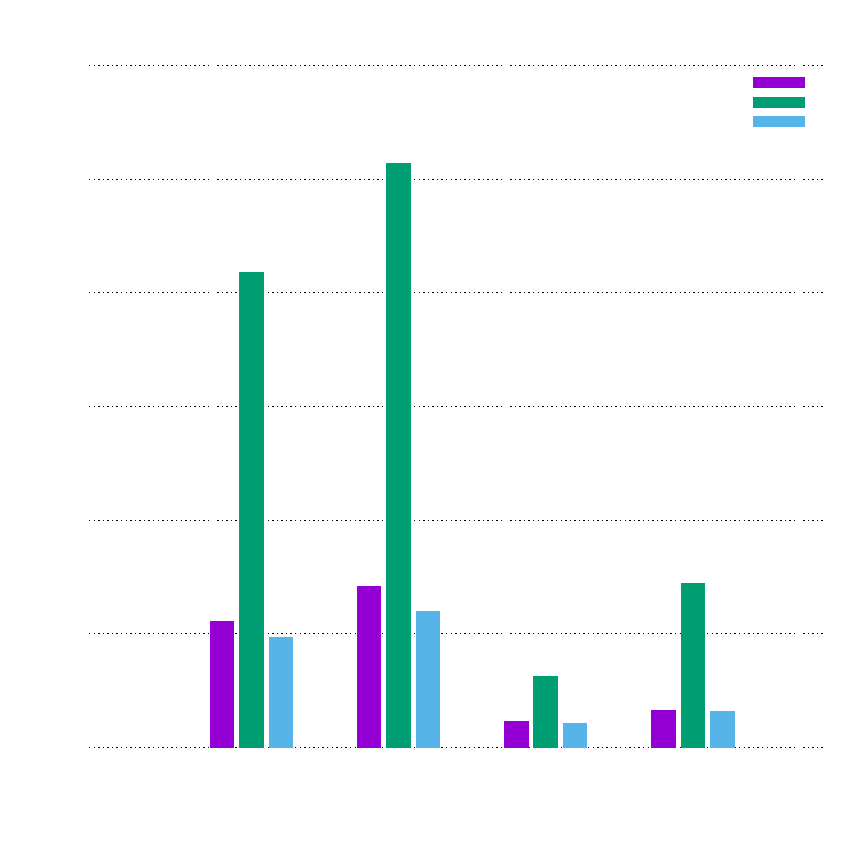
\includegraphics{euc_dist}}%
    \gplfronttext
  \end{picture}%
\endgroup

  \caption{Euclidean error scores (sum of euclidean distances for corresponding points) across the datasets. A threshold of $1.0$ has been used to cut-off fair laying point in non-overlapping areas, see section~\ref{sec:transform-evaluation} for details. The map-merging run with default parameters including \gls{PFH} descriptors and \gls{SIFT} keypoints. The first two scores are for initial estimation using descriptors matching, using my reciprocal matching scheme and \gls{SAC-IA} algorithm respectively (section~\ref{sec:matching}). The last score is the euclidean error after final refining with \gls{ICP} (section~\ref{sec:final-estimation}), the initial estimate from the reciprocal matching has been used for the \gls{ICP} refinement.}
  \label{fig:plot:euc_dist}
\end{figure}

Both ``Vicon Room'' datasets show very small Euclidean error, well beyond the size of one voxel ($0.05$ m).

The Euclidean error for the initial estimate is significantly lower for the presented reciprocal matching method (section~\ref{sec:matching}). For the \gls{SAC-IA} algorithm the error is higher because the randomness used in the algorithm introduces additional errors in case of well-performing \gls{PFH} descriptors. The initial estimate produced by the presented matching method is close to the final estimate refined with \gls{ICP}. The \gls{ICP} refinement is then very fast without negative impact on the overall time of the map-merging algorithm (figure~\ref{fig:plot:perf}).

\section{Estimation robustness}

Important measure of estimation robustness is the number of inliers (figure~\ref{fig:plot:inliers}) in the \gls{RANSAC} estimate (section~\ref{sec:transform-evaluation}). Inliers are the points which are ultimately used for computing transformation estimate. Estimates based on small number of inliers might be severely affected by the noise. On the other hand estimates based on large number of inliers, especially with high inliers ratio to all points, are supposed to be reasonably confident in typical applications.

\begin{figure}
  \centering
  % GNUPLOT: LaTeX picture with Postscript
\begingroup
  \makeatletter
  \providecommand\color[2][]{%
    \GenericError{(gnuplot) \space\space\space\@spaces}{%
      Package color not loaded in conjunction with
      terminal option `colourtext'%
    }{See the gnuplot documentation for explanation.%
    }{Either use 'blacktext' in gnuplot or load the package
      color.sty in LaTeX.}%
    \renewcommand\color[2][]{}%
  }%
  \providecommand\includegraphics[2][]{%
    \GenericError{(gnuplot) \space\space\space\@spaces}{%
      Package graphicx or graphics not loaded%
    }{See the gnuplot documentation for explanation.%
    }{The gnuplot epslatex terminal needs graphicx.sty or graphics.sty.}%
    \renewcommand\includegraphics[2][]{}%
  }%
  \providecommand\rotatebox[2]{#2}%
  \@ifundefined{ifGPcolor}{%
    \newif\ifGPcolor
    \GPcolortrue
  }{}%
  \@ifundefined{ifGPblacktext}{%
    \newif\ifGPblacktext
    \GPblacktextfalse
  }{}%
  % define a \g@addto@macro without @ in the name:
  \let\gplgaddtomacro\g@addto@macro
  % define empty templates for all commands taking text:
  \gdef\gplbacktext{}%
  \gdef\gplfronttext{}%
  \makeatother
  \ifGPblacktext
    % no textcolor at all
    \def\colorrgb#1{}%
    \def\colorgray#1{}%
  \else
    % gray or color?
    \ifGPcolor
      \def\colorrgb#1{\color[rgb]{#1}}%
      \def\colorgray#1{\color[gray]{#1}}%
      \expandafter\def\csname LTw\endcsname{\color{white}}%
      \expandafter\def\csname LTb\endcsname{\color{black}}%
      \expandafter\def\csname LTa\endcsname{\color{black}}%
      \expandafter\def\csname LT0\endcsname{\color[rgb]{1,0,0}}%
      \expandafter\def\csname LT1\endcsname{\color[rgb]{0,1,0}}%
      \expandafter\def\csname LT2\endcsname{\color[rgb]{0,0,1}}%
      \expandafter\def\csname LT3\endcsname{\color[rgb]{1,0,1}}%
      \expandafter\def\csname LT4\endcsname{\color[rgb]{0,1,1}}%
      \expandafter\def\csname LT5\endcsname{\color[rgb]{1,1,0}}%
      \expandafter\def\csname LT6\endcsname{\color[rgb]{0,0,0}}%
      \expandafter\def\csname LT7\endcsname{\color[rgb]{1,0.3,0}}%
      \expandafter\def\csname LT8\endcsname{\color[rgb]{0.5,0.5,0.5}}%
    \else
      % gray
      \def\colorrgb#1{\color{black}}%
      \def\colorgray#1{\color[gray]{#1}}%
      \expandafter\def\csname LTw\endcsname{\color{white}}%
      \expandafter\def\csname LTb\endcsname{\color{black}}%
      \expandafter\def\csname LTa\endcsname{\color{black}}%
      \expandafter\def\csname LT0\endcsname{\color{black}}%
      \expandafter\def\csname LT1\endcsname{\color{black}}%
      \expandafter\def\csname LT2\endcsname{\color{black}}%
      \expandafter\def\csname LT3\endcsname{\color{black}}%
      \expandafter\def\csname LT4\endcsname{\color{black}}%
      \expandafter\def\csname LT5\endcsname{\color{black}}%
      \expandafter\def\csname LT6\endcsname{\color{black}}%
      \expandafter\def\csname LT7\endcsname{\color{black}}%
      \expandafter\def\csname LT8\endcsname{\color{black}}%
    \fi
  \fi
    \setlength{\unitlength}{0.0500bp}%
    \ifx\gptboxheight\undefined%
      \newlength{\gptboxheight}%
      \newlength{\gptboxwidth}%
      \newsavebox{\gptboxtext}%
    \fi%
    \setlength{\fboxrule}{0.5pt}%
    \setlength{\fboxsep}{1pt}%
\begin{picture}(8220.00,8220.00)%
    \gplgaddtomacro\gplbacktext{%
      \csname LTb\endcsname%%
      \put(459,1051){\makebox(0,0)[r]{\strut{}$0$}}%
      \csname LTb\endcsname%%
      \put(459,1646){\makebox(0,0)[r]{\strut{}$50$}}%
      \csname LTb\endcsname%%
      \put(459,2242){\makebox(0,0)[r]{\strut{}$100$}}%
      \csname LTb\endcsname%%
      \put(459,2837){\makebox(0,0)[r]{\strut{}$150$}}%
      \csname LTb\endcsname%%
      \put(459,3432){\makebox(0,0)[r]{\strut{}$200$}}%
      \csname LTb\endcsname%%
      \put(459,4027){\makebox(0,0)[r]{\strut{}$250$}}%
      \csname LTb\endcsname%%
      \put(459,4623){\makebox(0,0)[r]{\strut{}$300$}}%
      \csname LTb\endcsname%%
      \put(459,5218){\makebox(0,0)[r]{\strut{}$350$}}%
      \csname LTb\endcsname%%
      \put(459,5813){\makebox(0,0)[r]{\strut{}$400$}}%
      \csname LTb\endcsname%%
      \put(459,6408){\makebox(0,0)[r]{\strut{}$450$}}%
      \csname LTb\endcsname%%
      \put(459,7004){\makebox(0,0)[r]{\strut{}$500$}}%
      \csname LTb\endcsname%%
      \put(459,7599){\makebox(0,0)[r]{\strut{}$550$}}%
      \csname LTb\endcsname%%
      \put(2031,949){\rotatebox{-45}{\makebox(0,0)[l]{\strut{}AAU forest}}}%
      \csname LTb\endcsname%%
      \put(3502,949){\rotatebox{-45}{\makebox(0,0)[l]{\strut{}Machine Hall}}}%
      \csname LTb\endcsname%%
      \put(4972,949){\rotatebox{-45}{\makebox(0,0)[l]{\strut{}Vicon Room 1}}}%
      \csname LTb\endcsname%%
      \put(6443,949){\rotatebox{-45}{\makebox(0,0)[l]{\strut{}Vicon Room 2}}}%
    }%
    \gplgaddtomacro\gplfronttext{%
      \csname LTb\endcsname%%
      \put(4237,7940){\makebox(0,0){\strut{}Number of matches and inliers}}%
      \csname LTb\endcsname%%
      \put(7125,7432){\makebox(0,0)[r]{\strut{}cross-matches count}}%
      \csname LTb\endcsname%%
      \put(7125,7246){\makebox(0,0)[r]{\strut{}inliers count}}%
      \csname LTb\endcsname%%
      \put(2378,1392){\makebox(0,0){\strut{}13}}%
      \csname LTb\endcsname%%
      \put(3849,1511){\makebox(0,0){\strut{}23}}%
      \csname LTb\endcsname%%
      \put(5319,1666){\makebox(0,0){\strut{}36}}%
      \csname LTb\endcsname%%
      \put(6790,1356){\makebox(0,0){\strut{}10}}%
    }%
    \gplbacktext
    \put(0,0){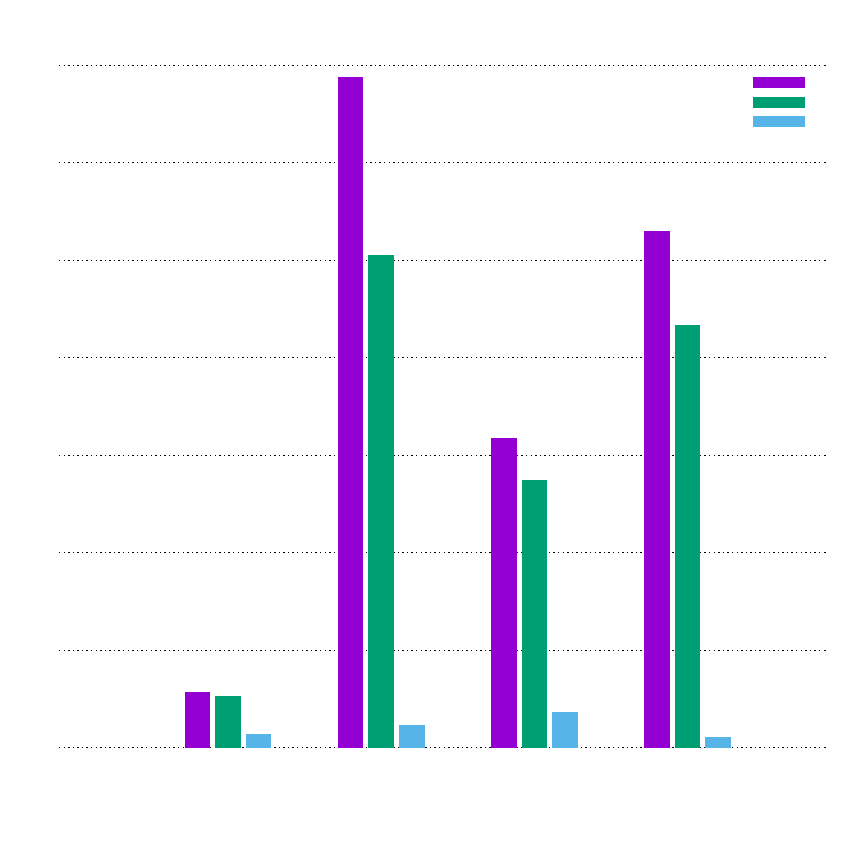
\includegraphics{inliers}}%
    \gplfronttext
  \end{picture}%
\endgroup

  \caption{Number of keypoints, descriptor matches and number of inliers across the datasets with default parameters. Default parameters include \gls{PFH} descriptors and \gls{SIFT} keypoints. The reciprocal matching algorithm (section~\ref{sec:matching}) has been used for matching. Keypoints are shown for the first map of each environment.}
  \label{fig:plot:inliers}
\end{figure}

The inlier ratio to number of matches is quite low, even for \gls{PFH} descriptors (figure~\ref{fig:plot:inliers}), the similar ratios has been observed for all the descriptors. This is partially caused by the matching scheme designed to accept also more distant matches to improve inlier ratio for less descriptive descriptors as discussed din section~\ref{sec:matching}. The same behaviour causes number of matches to be relatively high compared to number of keypoints (figure~\ref{fig:plot:inliers}).

The ``AAU forest'' and ``Vicon Room 2'' datasets have low numbers of inliers, which might impact robustness in such environments. The ``AAU forest'' is a relatively small, difficult environment for mapping containing noise and mapping errors. Only a few regions in maps are suitable for producing reliable matching points, which leads to small number of inliers.

For the ``Vicon Room 2'' dataset colour-based descriptors exhibited generally better performance (figure~\ref{fig:plot:desc_inliers}) allow robust estimation for this dataset. The ``Vicon Room 2'' maps also contain noise caused by the dynamic motion of the aerial vehicle.

Interestingly in both cases with limited number of inliers, the map-merging algorithm has been able to produce an accurate merge (figure~\ref{fig:plot:euc_dist}), even before \gls{ICP} refining. The inliers proved to be the correct matches.

\section{Descriptors}

As already noted in the previous section, the performance of the descriptors varies significantly in some cases (figure~\ref{fig:plot:desc_inliers}). The \gls{PFHRGB} descriptors exhibited the highest number of inliers across the datasets (figure~\ref{fig:plot:desc_inliers}). The \gls{SHOT} descriptors with colour also exhibited decent amount of inliers, especially considering the fast processing speed (section~\ref{sec:runtime-perf}).

\begin{figure}
  \centering
  % GNUPLOT: LaTeX picture with Postscript
\begingroup
  \makeatletter
  \providecommand\color[2][]{%
    \GenericError{(gnuplot) \space\space\space\@spaces}{%
      Package color not loaded in conjunction with
      terminal option `colourtext'%
    }{See the gnuplot documentation for explanation.%
    }{Either use 'blacktext' in gnuplot or load the package
      color.sty in LaTeX.}%
    \renewcommand\color[2][]{}%
  }%
  \providecommand\includegraphics[2][]{%
    \GenericError{(gnuplot) \space\space\space\@spaces}{%
      Package graphicx or graphics not loaded%
    }{See the gnuplot documentation for explanation.%
    }{The gnuplot epslatex terminal needs graphicx.sty or graphics.sty.}%
    \renewcommand\includegraphics[2][]{}%
  }%
  \providecommand\rotatebox[2]{#2}%
  \@ifundefined{ifGPcolor}{%
    \newif\ifGPcolor
    \GPcolortrue
  }{}%
  \@ifundefined{ifGPblacktext}{%
    \newif\ifGPblacktext
    \GPblacktextfalse
  }{}%
  % define a \g@addto@macro without @ in the name:
  \let\gplgaddtomacro\g@addto@macro
  % define empty templates for all commands taking text:
  \gdef\gplbacktext{}%
  \gdef\gplfronttext{}%
  \makeatother
  \ifGPblacktext
    % no textcolor at all
    \def\colorrgb#1{}%
    \def\colorgray#1{}%
  \else
    % gray or color?
    \ifGPcolor
      \def\colorrgb#1{\color[rgb]{#1}}%
      \def\colorgray#1{\color[gray]{#1}}%
      \expandafter\def\csname LTw\endcsname{\color{white}}%
      \expandafter\def\csname LTb\endcsname{\color{black}}%
      \expandafter\def\csname LTa\endcsname{\color{black}}%
      \expandafter\def\csname LT0\endcsname{\color[rgb]{1,0,0}}%
      \expandafter\def\csname LT1\endcsname{\color[rgb]{0,1,0}}%
      \expandafter\def\csname LT2\endcsname{\color[rgb]{0,0,1}}%
      \expandafter\def\csname LT3\endcsname{\color[rgb]{1,0,1}}%
      \expandafter\def\csname LT4\endcsname{\color[rgb]{0,1,1}}%
      \expandafter\def\csname LT5\endcsname{\color[rgb]{1,1,0}}%
      \expandafter\def\csname LT6\endcsname{\color[rgb]{0,0,0}}%
      \expandafter\def\csname LT7\endcsname{\color[rgb]{1,0.3,0}}%
      \expandafter\def\csname LT8\endcsname{\color[rgb]{0.5,0.5,0.5}}%
    \else
      % gray
      \def\colorrgb#1{\color{black}}%
      \def\colorgray#1{\color[gray]{#1}}%
      \expandafter\def\csname LTw\endcsname{\color{white}}%
      \expandafter\def\csname LTb\endcsname{\color{black}}%
      \expandafter\def\csname LTa\endcsname{\color{black}}%
      \expandafter\def\csname LT0\endcsname{\color{black}}%
      \expandafter\def\csname LT1\endcsname{\color{black}}%
      \expandafter\def\csname LT2\endcsname{\color{black}}%
      \expandafter\def\csname LT3\endcsname{\color{black}}%
      \expandafter\def\csname LT4\endcsname{\color{black}}%
      \expandafter\def\csname LT5\endcsname{\color{black}}%
      \expandafter\def\csname LT6\endcsname{\color{black}}%
      \expandafter\def\csname LT7\endcsname{\color{black}}%
      \expandafter\def\csname LT8\endcsname{\color{black}}%
    \fi
  \fi
    \setlength{\unitlength}{0.0500bp}%
    \ifx\gptboxheight\undefined%
      \newlength{\gptboxheight}%
      \newlength{\gptboxwidth}%
      \newsavebox{\gptboxtext}%
    \fi%
    \setlength{\fboxrule}{0.5pt}%
    \setlength{\fboxsep}{1pt}%
\begin{picture}(8220.00,8220.00)%
    \gplgaddtomacro\gplbacktext{%
      \csname LTb\endcsname%%
      \put(357,1051){\makebox(0,0)[r]{\strut{}$0$}}%
      \csname LTb\endcsname%%
      \put(357,1779){\makebox(0,0)[r]{\strut{}$5$}}%
      \csname LTb\endcsname%%
      \put(357,2506){\makebox(0,0)[r]{\strut{}$10$}}%
      \csname LTb\endcsname%%
      \put(357,3234){\makebox(0,0)[r]{\strut{}$15$}}%
      \csname LTb\endcsname%%
      \put(357,3961){\makebox(0,0)[r]{\strut{}$20$}}%
      \csname LTb\endcsname%%
      \put(357,4689){\makebox(0,0)[r]{\strut{}$25$}}%
      \csname LTb\endcsname%%
      \put(357,5416){\makebox(0,0)[r]{\strut{}$30$}}%
      \csname LTb\endcsname%%
      \put(357,6144){\makebox(0,0)[r]{\strut{}$35$}}%
      \csname LTb\endcsname%%
      \put(357,6871){\makebox(0,0)[r]{\strut{}$40$}}%
      \csname LTb\endcsname%%
      \put(357,7599){\makebox(0,0)[r]{\strut{}$45$}}%
      \csname LTb\endcsname%%
      \put(1950,949){\rotatebox{-45}{\makebox(0,0)[l]{\strut{}AAU forest}}}%
      \csname LTb\endcsname%%
      \put(3441,949){\rotatebox{-45}{\makebox(0,0)[l]{\strut{}Machine Hall}}}%
      \csname LTb\endcsname%%
      \put(4931,949){\rotatebox{-45}{\makebox(0,0)[l]{\strut{}Vicon Room 1}}}%
      \csname LTb\endcsname%%
      \put(6422,949){\rotatebox{-45}{\makebox(0,0)[l]{\strut{}Vicon Room 2}}}%
    }%
    \gplgaddtomacro\gplfronttext{%
      \csname LTb\endcsname%%
      \put(4186,7940){\makebox(0,0){\strut{}Number of inliers per descriptor}}%
      \csname LTb\endcsname%%
      \put(1173,7432){\makebox(0,0)[r]{\strut{}FPFH}}%
      \csname LTb\endcsname%%
      \put(1173,7246){\makebox(0,0)[r]{\strut{}PFH}}%
      \csname LTb\endcsname%%
      \put(1173,7060){\makebox(0,0)[r]{\strut{}PFHRGB}}%
      \csname LTb\endcsname%%
      \put(1173,6874){\makebox(0,0)[r]{\strut{}SC3D}}%
      \csname LTb\endcsname%%
      \put(1173,6688){\makebox(0,0)[r]{\strut{}SHOT}}%
    }%
    \gplbacktext
    \put(0,0){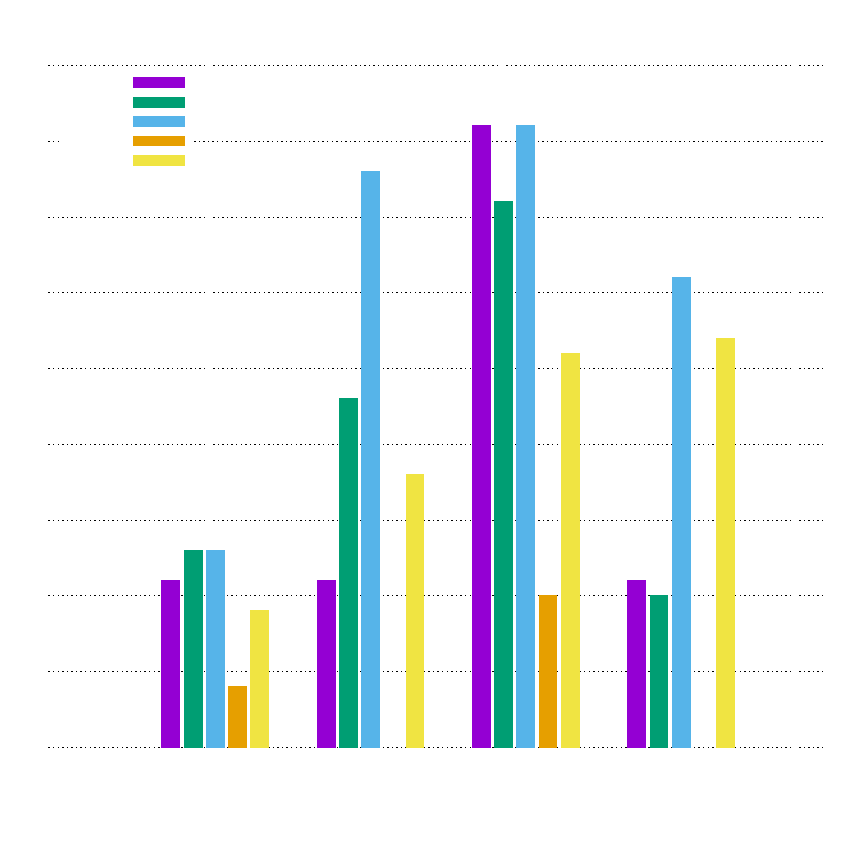
\includegraphics{desc_inliers}}%
    \gplfronttext
  \end{picture}%
\endgroup

  \caption{Number of inliers across the datasets for different descriptor algorithms. Apart from descriptors algorithms, the default parameters has been used including \gls{SIFT} keypoints and the reciprocal matching algorithm (section~\ref{sec:matching}). The \gls{PCL} implementation of \gls{SC3D} descriptors crashed on ``Machine Hall'' and ``Vicon Room 2'' datasets. This might indicate that the implementation in \gls{PCL} is probably not as mature as the remaining descriptors, but I have not investigated further.}
  \label{fig:plot:desc_inliers}
\end{figure}

The lowest number of inliers have been produced by \gls{SC3D} descriptors. Moreover the \gls{PCL} implementation of \gls{SC3D} crashed in two instances. Together with \gls{RSD} descriptors, which has not been able to produce any inliers and are not shown in the plots, the \gls{SC3D} may not be suitable for map-merging in the evaluated setup.

Euclidean error distances (figure~\ref{fig:plot:desc_dist}) mostly reflects number of inliers for respective descriptors, with \gls{PFHRGB} descriptors generally providing the best initial transformation. With one exception, the \gls{ICP} refining was able to produce high-quality alignment for all descriptors with small error differences, neglecting the differences between initial alignments for different descriptors. For the \gls{FPFH} descriptors the initial estimate in ``Machine Hall'' dataset has significantly higher error and the \gls{ICP} refining stuck in the local extreme.

\begin{figure}
  \centering
  % GNUPLOT: LaTeX picture with Postscript
\begingroup
  \makeatletter
  \providecommand\color[2][]{%
    \GenericError{(gnuplot) \space\space\space\@spaces}{%
      Package color not loaded in conjunction with
      terminal option `colourtext'%
    }{See the gnuplot documentation for explanation.%
    }{Either use 'blacktext' in gnuplot or load the package
      color.sty in LaTeX.}%
    \renewcommand\color[2][]{}%
  }%
  \providecommand\includegraphics[2][]{%
    \GenericError{(gnuplot) \space\space\space\@spaces}{%
      Package graphicx or graphics not loaded%
    }{See the gnuplot documentation for explanation.%
    }{The gnuplot epslatex terminal needs graphicx.sty or graphics.sty.}%
    \renewcommand\includegraphics[2][]{}%
  }%
  \providecommand\rotatebox[2]{#2}%
  \@ifundefined{ifGPcolor}{%
    \newif\ifGPcolor
    \GPcolortrue
  }{}%
  \@ifundefined{ifGPblacktext}{%
    \newif\ifGPblacktext
    \GPblacktextfalse
  }{}%
  % define a \g@addto@macro without @ in the name:
  \let\gplgaddtomacro\g@addto@macro
  % define empty templates for all commands taking text:
  \gdef\gplbacktext{}%
  \gdef\gplfronttext{}%
  \makeatother
  \ifGPblacktext
    % no textcolor at all
    \def\colorrgb#1{}%
    \def\colorgray#1{}%
  \else
    % gray or color?
    \ifGPcolor
      \def\colorrgb#1{\color[rgb]{#1}}%
      \def\colorgray#1{\color[gray]{#1}}%
      \expandafter\def\csname LTw\endcsname{\color{white}}%
      \expandafter\def\csname LTb\endcsname{\color{black}}%
      \expandafter\def\csname LTa\endcsname{\color{black}}%
      \expandafter\def\csname LT0\endcsname{\color[rgb]{1,0,0}}%
      \expandafter\def\csname LT1\endcsname{\color[rgb]{0,1,0}}%
      \expandafter\def\csname LT2\endcsname{\color[rgb]{0,0,1}}%
      \expandafter\def\csname LT3\endcsname{\color[rgb]{1,0,1}}%
      \expandafter\def\csname LT4\endcsname{\color[rgb]{0,1,1}}%
      \expandafter\def\csname LT5\endcsname{\color[rgb]{1,1,0}}%
      \expandafter\def\csname LT6\endcsname{\color[rgb]{0,0,0}}%
      \expandafter\def\csname LT7\endcsname{\color[rgb]{1,0.3,0}}%
      \expandafter\def\csname LT8\endcsname{\color[rgb]{0.5,0.5,0.5}}%
    \else
      % gray
      \def\colorrgb#1{\color{black}}%
      \def\colorgray#1{\color[gray]{#1}}%
      \expandafter\def\csname LTw\endcsname{\color{white}}%
      \expandafter\def\csname LTb\endcsname{\color{black}}%
      \expandafter\def\csname LTa\endcsname{\color{black}}%
      \expandafter\def\csname LT0\endcsname{\color{black}}%
      \expandafter\def\csname LT1\endcsname{\color{black}}%
      \expandafter\def\csname LT2\endcsname{\color{black}}%
      \expandafter\def\csname LT3\endcsname{\color{black}}%
      \expandafter\def\csname LT4\endcsname{\color{black}}%
      \expandafter\def\csname LT5\endcsname{\color{black}}%
      \expandafter\def\csname LT6\endcsname{\color{black}}%
      \expandafter\def\csname LT7\endcsname{\color{black}}%
      \expandafter\def\csname LT8\endcsname{\color{black}}%
    \fi
  \fi
    \setlength{\unitlength}{0.0500bp}%
    \ifx\gptboxheight\undefined%
      \newlength{\gptboxheight}%
      \newlength{\gptboxwidth}%
      \newsavebox{\gptboxtext}%
    \fi%
    \setlength{\fboxrule}{0.5pt}%
    \setlength{\fboxsep}{1pt}%
\begin{picture}(8220.00,8220.00)%
    \gplgaddtomacro\gplbacktext{%
      \csname LTb\endcsname%%
      \put(747,1051){\makebox(0,0)[r]{\strut{}$0$}}%
      \csname LTb\endcsname%%
      \put(747,1986){\makebox(0,0)[r]{\strut{}$0.05$}}%
      \csname LTb\endcsname%%
      \put(747,2922){\makebox(0,0)[r]{\strut{}$0.1$}}%
      \csname LTb\endcsname%%
      \put(747,3857){\makebox(0,0)[r]{\strut{}$0.15$}}%
      \csname LTb\endcsname%%
      \put(747,4793){\makebox(0,0)[r]{\strut{}$0.2$}}%
      \csname LTb\endcsname%%
      \put(747,5728){\makebox(0,0)[r]{\strut{}$0.25$}}%
      \csname LTb\endcsname%%
      \put(747,6664){\makebox(0,0)[r]{\strut{}$0.3$}}%
      \csname LTb\endcsname%%
      \put(747,7599){\makebox(0,0)[r]{\strut{}$0.35$}}%
      \csname LTb\endcsname%%
      \put(2262,949){\rotatebox{-45}{\makebox(0,0)[l]{\strut{}AAU forest}}}%
      \csname LTb\endcsname%%
      \put(3675,949){\rotatebox{-45}{\makebox(0,0)[l]{\strut{}Machine Hall}}}%
      \csname LTb\endcsname%%
      \put(5087,949){\rotatebox{-45}{\makebox(0,0)[l]{\strut{}Vicon Room 1}}}%
      \csname LTb\endcsname%%
      \put(6500,949){\rotatebox{-45}{\makebox(0,0)[l]{\strut{}Vicon Room 2}}}%
    }%
    \gplgaddtomacro\gplfronttext{%
      \csname LTb\endcsname%%
      \put(153,4325){\rotatebox{-270}{\makebox(0,0){\strut{}Distance (m)}}}%
      \csname LTb\endcsname%%
      \put(4381,7940){\makebox(0,0){\strut{}Euclidean error distance for descriptors}}%
      \csname LTb\endcsname%%
      \put(7125,7432){\makebox(0,0)[r]{\strut{}FPFH}}%
      \csname LTb\endcsname%%
      \put(7125,7246){\makebox(0,0)[r]{\strut{}PFH}}%
      \csname LTb\endcsname%%
      \put(7125,7060){\makebox(0,0)[r]{\strut{}PFHRGB}}%
      \csname LTb\endcsname%%
      \put(7125,6874){\makebox(0,0)[r]{\strut{}SC3D}}%
      \csname LTb\endcsname%%
      \put(7125,6688){\makebox(0,0)[r]{\strut{}SHOT}}%
      \csname LTb\endcsname%%
      \put(7125,6502){\makebox(0,0)[r]{\strut{}MATCHING}}%
      \csname LTb\endcsname%%
      \put(7125,6316){\makebox(0,0)[r]{\strut{}SAC-IA}}%
      \csname LTb\endcsname%%
      \put(7125,6130){\makebox(0,0)[r]{\strut{}ICP}}%
    }%
    \gplbacktext
    \put(0,0){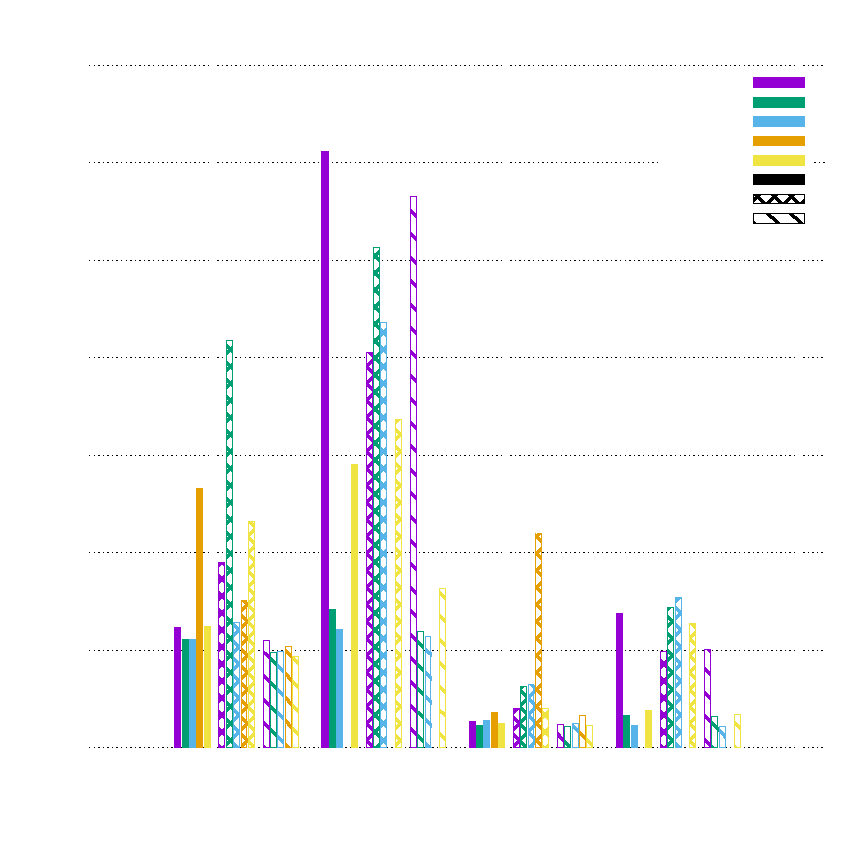
\includegraphics{desc_dist}}%
    \gplfronttext
  \end{picture}%
\endgroup

  \caption{Euclidean error scores (sum of euclidean distances for corresponding points) across the datasets for different descriptor algorithms. Similarly to figure~\ref{fig:plot:euc_dist} the first two scores are for the initial estimates, using the reciprocal matching algorithm and the \gls{SAC-IA} respectively, the last score is for the final refining with \gls{ICP}, using initial estimate from the reciprocal matching algorithm.}
  \label{fig:plot:desc_dist}
\end{figure}

\section{Runtime performance}
\label{sec:runtime-perf}

Although the runtime performance was not a primary concern of the presented algorithm, it is interesting to take a look on the processing time. In the default configuration (figure~\ref{fig:plot:perf}), there are order of magnitude differences between algorithm steps as presented in section~\ref{sec:estimate-pair-wise}. Most of the processing time is taken by the \gls{SIFT} keypoints detection and computation of \gls{PFH} descriptors.

\begin{figure}
  \centering
  % GNUPLOT: LaTeX picture with Postscript
\begingroup
  \makeatletter
  \providecommand\color[2][]{%
    \GenericError{(gnuplot) \space\space\space\@spaces}{%
      Package color not loaded in conjunction with
      terminal option `colourtext'%
    }{See the gnuplot documentation for explanation.%
    }{Either use 'blacktext' in gnuplot or load the package
      color.sty in LaTeX.}%
    \renewcommand\color[2][]{}%
  }%
  \providecommand\includegraphics[2][]{%
    \GenericError{(gnuplot) \space\space\space\@spaces}{%
      Package graphicx or graphics not loaded%
    }{See the gnuplot documentation for explanation.%
    }{The gnuplot epslatex terminal needs graphicx.sty or graphics.sty.}%
    \renewcommand\includegraphics[2][]{}%
  }%
  \providecommand\rotatebox[2]{#2}%
  \@ifundefined{ifGPcolor}{%
    \newif\ifGPcolor
    \GPcolortrue
  }{}%
  \@ifundefined{ifGPblacktext}{%
    \newif\ifGPblacktext
    \GPblacktextfalse
  }{}%
  % define a \g@addto@macro without @ in the name:
  \let\gplgaddtomacro\g@addto@macro
  % define empty templates for all commands taking text:
  \gdef\gplbacktext{}%
  \gdef\gplfronttext{}%
  \makeatother
  \ifGPblacktext
    % no textcolor at all
    \def\colorrgb#1{}%
    \def\colorgray#1{}%
  \else
    % gray or color?
    \ifGPcolor
      \def\colorrgb#1{\color[rgb]{#1}}%
      \def\colorgray#1{\color[gray]{#1}}%
      \expandafter\def\csname LTw\endcsname{\color{white}}%
      \expandafter\def\csname LTb\endcsname{\color{black}}%
      \expandafter\def\csname LTa\endcsname{\color{black}}%
      \expandafter\def\csname LT0\endcsname{\color[rgb]{1,0,0}}%
      \expandafter\def\csname LT1\endcsname{\color[rgb]{0,1,0}}%
      \expandafter\def\csname LT2\endcsname{\color[rgb]{0,0,1}}%
      \expandafter\def\csname LT3\endcsname{\color[rgb]{1,0,1}}%
      \expandafter\def\csname LT4\endcsname{\color[rgb]{0,1,1}}%
      \expandafter\def\csname LT5\endcsname{\color[rgb]{1,1,0}}%
      \expandafter\def\csname LT6\endcsname{\color[rgb]{0,0,0}}%
      \expandafter\def\csname LT7\endcsname{\color[rgb]{1,0.3,0}}%
      \expandafter\def\csname LT8\endcsname{\color[rgb]{0.5,0.5,0.5}}%
    \else
      % gray
      \def\colorrgb#1{\color{black}}%
      \def\colorgray#1{\color[gray]{#1}}%
      \expandafter\def\csname LTw\endcsname{\color{white}}%
      \expandafter\def\csname LTb\endcsname{\color{black}}%
      \expandafter\def\csname LTa\endcsname{\color{black}}%
      \expandafter\def\csname LT0\endcsname{\color{black}}%
      \expandafter\def\csname LT1\endcsname{\color{black}}%
      \expandafter\def\csname LT2\endcsname{\color{black}}%
      \expandafter\def\csname LT3\endcsname{\color{black}}%
      \expandafter\def\csname LT4\endcsname{\color{black}}%
      \expandafter\def\csname LT5\endcsname{\color{black}}%
      \expandafter\def\csname LT6\endcsname{\color{black}}%
      \expandafter\def\csname LT7\endcsname{\color{black}}%
      \expandafter\def\csname LT8\endcsname{\color{black}}%
    \fi
  \fi
    \setlength{\unitlength}{0.0500bp}%
    \ifx\gptboxheight\undefined%
      \newlength{\gptboxheight}%
      \newlength{\gptboxwidth}%
      \newsavebox{\gptboxtext}%
    \fi%
    \setlength{\fboxrule}{0.5pt}%
    \setlength{\fboxsep}{1pt}%
\begin{picture}(8220.00,8220.00)%
    \gplgaddtomacro\gplbacktext{%
      \csname LTb\endcsname%%
      \put(849,1051){\makebox(0,0)[r]{\strut{}$0$}}%
      \csname LTb\endcsname%%
      \put(849,1870){\makebox(0,0)[r]{\strut{}$10000$}}%
      \csname LTb\endcsname%%
      \put(849,2688){\makebox(0,0)[r]{\strut{}$20000$}}%
      \csname LTb\endcsname%%
      \put(849,3507){\makebox(0,0)[r]{\strut{}$30000$}}%
      \csname LTb\endcsname%%
      \put(849,4325){\makebox(0,0)[r]{\strut{}$40000$}}%
      \csname LTb\endcsname%%
      \put(849,5144){\makebox(0,0)[r]{\strut{}$50000$}}%
      \csname LTb\endcsname%%
      \put(849,5962){\makebox(0,0)[r]{\strut{}$60000$}}%
      \csname LTb\endcsname%%
      \put(849,6781){\makebox(0,0)[r]{\strut{}$70000$}}%
      \csname LTb\endcsname%%
      \put(849,7599){\makebox(0,0)[r]{\strut{}$80000$}}%
      \csname LTb\endcsname%%
      \put(2343,949){\rotatebox{-45}{\makebox(0,0)[l]{\strut{}AAU forest}}}%
      \csname LTb\endcsname%%
      \put(3736,949){\rotatebox{-45}{\makebox(0,0)[l]{\strut{}Machine Hall}}}%
      \csname LTb\endcsname%%
      \put(5128,949){\rotatebox{-45}{\makebox(0,0)[l]{\strut{}Vicon Room 1}}}%
      \csname LTb\endcsname%%
      \put(6521,949){\rotatebox{-45}{\makebox(0,0)[l]{\strut{}Vicon Room 2}}}%
    }%
    \gplgaddtomacro\gplfronttext{%
      \csname LTb\endcsname%%
      \put(153,4325){\rotatebox{-270}{\makebox(0,0){\strut{}Time (ms)}}}%
      \csname LTb\endcsname%%
      \put(4432,7940){\makebox(0,0){\strut{}Performace}}%
      \csname LTb\endcsname%%
      \put(3399,7432){\makebox(0,0)[r]{\strut{}downsampling}}%
      \csname LTb\endcsname%%
      \put(3399,7246){\makebox(0,0)[r]{\strut{}removing outliers}}%
      \csname LTb\endcsname%%
      \put(3399,7060){\makebox(0,0)[r]{\strut{}normals computation}}%
      \csname LTb\endcsname%%
      \put(3399,6874){\makebox(0,0)[r]{\strut{}keypoints detection}}%
      \csname LTb\endcsname%%
      \put(3399,6688){\makebox(0,0)[r]{\strut{}descriptors computation}}%
      \csname LTb\endcsname%%
      \put(3399,6502){\makebox(0,0)[r]{\strut{}finding correspondences}}%
      \csname LTb\endcsname%%
      \put(3399,6316){\makebox(0,0)[r]{\strut{}ICP alignment}}%
    }%
    \gplbacktext
    \put(0,0){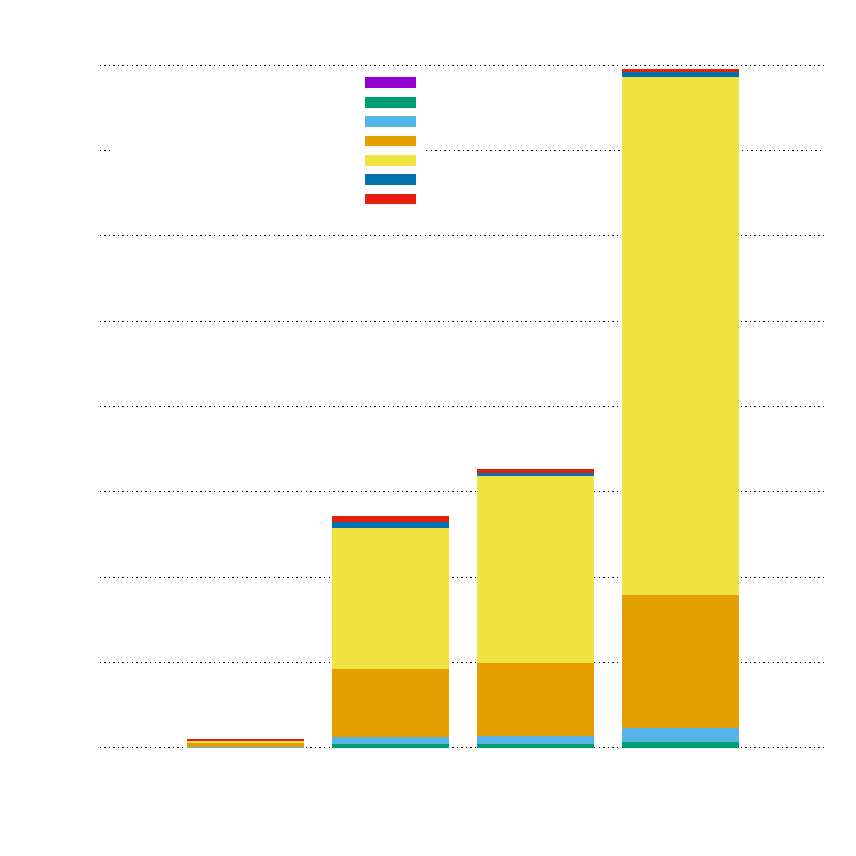
\includegraphics{perf}}%
    \gplfronttext
  \end{picture}%
\endgroup

  \caption{Runtime performance characteristics for the respective parts of the map-merging algorithm (section~\ref{sec:estimate-pair-wise}) across the datasets. The data has been recorded during one run of the algorithm on Intel(R) Core(TM) i5-2520M and do not incorporate measurements from multiple runs to deal with various sources of non-determinism, although the runtime of the algorithm has been observed to be quite stable. The data are intended to show order of magnitude differences of processing time between particular parts of the algorithm. The map-merging algorithm has been run with default parameters including \gls{PFH} descriptors and \gls{SIFT} keypoints.}
  \label{fig:plot:perf}
\end{figure}

There are, however, significant differences between descriptors regarding processing time (figure~\ref{fig:plot:desc_perf}). All \gls{PFH}-family descriptors require order of magnitude higher processing time. There are also significant differences between the \gls{PFH}-family, the processing time nearly doubles between \gls{FPFH}, \gls{PFH} and \gls{PFHRGB} descriptors.

The \gls{SHOT} descriptors with colour are very fast, which makes them compelling choice, considering also they showed good robustness (figure~\ref{fig:plot:desc_inliers}). \gls{PFHRGB} descriptors exhibited the best robustness, but also the longest processing time.

\begin{figure}
  \centering
  % GNUPLOT: LaTeX picture with Postscript
\begingroup
  \makeatletter
  \providecommand\color[2][]{%
    \GenericError{(gnuplot) \space\space\space\@spaces}{%
      Package color not loaded in conjunction with
      terminal option `colourtext'%
    }{See the gnuplot documentation for explanation.%
    }{Either use 'blacktext' in gnuplot or load the package
      color.sty in LaTeX.}%
    \renewcommand\color[2][]{}%
  }%
  \providecommand\includegraphics[2][]{%
    \GenericError{(gnuplot) \space\space\space\@spaces}{%
      Package graphicx or graphics not loaded%
    }{See the gnuplot documentation for explanation.%
    }{The gnuplot epslatex terminal needs graphicx.sty or graphics.sty.}%
    \renewcommand\includegraphics[2][]{}%
  }%
  \providecommand\rotatebox[2]{#2}%
  \@ifundefined{ifGPcolor}{%
    \newif\ifGPcolor
    \GPcolortrue
  }{}%
  \@ifundefined{ifGPblacktext}{%
    \newif\ifGPblacktext
    \GPblacktextfalse
  }{}%
  % define a \g@addto@macro without @ in the name:
  \let\gplgaddtomacro\g@addto@macro
  % define empty templates for all commands taking text:
  \gdef\gplbacktext{}%
  \gdef\gplfronttext{}%
  \makeatother
  \ifGPblacktext
    % no textcolor at all
    \def\colorrgb#1{}%
    \def\colorgray#1{}%
  \else
    % gray or color?
    \ifGPcolor
      \def\colorrgb#1{\color[rgb]{#1}}%
      \def\colorgray#1{\color[gray]{#1}}%
      \expandafter\def\csname LTw\endcsname{\color{white}}%
      \expandafter\def\csname LTb\endcsname{\color{black}}%
      \expandafter\def\csname LTa\endcsname{\color{black}}%
      \expandafter\def\csname LT0\endcsname{\color[rgb]{1,0,0}}%
      \expandafter\def\csname LT1\endcsname{\color[rgb]{0,1,0}}%
      \expandafter\def\csname LT2\endcsname{\color[rgb]{0,0,1}}%
      \expandafter\def\csname LT3\endcsname{\color[rgb]{1,0,1}}%
      \expandafter\def\csname LT4\endcsname{\color[rgb]{0,1,1}}%
      \expandafter\def\csname LT5\endcsname{\color[rgb]{1,1,0}}%
      \expandafter\def\csname LT6\endcsname{\color[rgb]{0,0,0}}%
      \expandafter\def\csname LT7\endcsname{\color[rgb]{1,0.3,0}}%
      \expandafter\def\csname LT8\endcsname{\color[rgb]{0.5,0.5,0.5}}%
    \else
      % gray
      \def\colorrgb#1{\color{black}}%
      \def\colorgray#1{\color[gray]{#1}}%
      \expandafter\def\csname LTw\endcsname{\color{white}}%
      \expandafter\def\csname LTb\endcsname{\color{black}}%
      \expandafter\def\csname LTa\endcsname{\color{black}}%
      \expandafter\def\csname LT0\endcsname{\color{black}}%
      \expandafter\def\csname LT1\endcsname{\color{black}}%
      \expandafter\def\csname LT2\endcsname{\color{black}}%
      \expandafter\def\csname LT3\endcsname{\color{black}}%
      \expandafter\def\csname LT4\endcsname{\color{black}}%
      \expandafter\def\csname LT5\endcsname{\color{black}}%
      \expandafter\def\csname LT6\endcsname{\color{black}}%
      \expandafter\def\csname LT7\endcsname{\color{black}}%
      \expandafter\def\csname LT8\endcsname{\color{black}}%
    \fi
  \fi
    \setlength{\unitlength}{0.0500bp}%
    \ifx\gptboxheight\undefined%
      \newlength{\gptboxheight}%
      \newlength{\gptboxwidth}%
      \newsavebox{\gptboxtext}%
    \fi%
    \setlength{\fboxrule}{0.5pt}%
    \setlength{\fboxsep}{1pt}%
\begin{picture}(8220.00,8220.00)%
    \gplgaddtomacro\gplbacktext{%
      \csname LTb\endcsname%%
      \put(951,1051){\makebox(0,0)[r]{\strut{}$0$}}%
      \csname LTb\endcsname%%
      \put(951,2142){\makebox(0,0)[r]{\strut{}$20000$}}%
      \csname LTb\endcsname%%
      \put(951,3234){\makebox(0,0)[r]{\strut{}$40000$}}%
      \csname LTb\endcsname%%
      \put(951,4325){\makebox(0,0)[r]{\strut{}$60000$}}%
      \csname LTb\endcsname%%
      \put(951,5416){\makebox(0,0)[r]{\strut{}$80000$}}%
      \csname LTb\endcsname%%
      \put(951,6508){\makebox(0,0)[r]{\strut{}$100000$}}%
      \csname LTb\endcsname%%
      \put(951,7599){\makebox(0,0)[r]{\strut{}$120000$}}%
      \csname LTb\endcsname%%
      \put(2425,949){\rotatebox{-45}{\makebox(0,0)[l]{\strut{}AAU forest}}}%
      \csname LTb\endcsname%%
      \put(3797,949){\rotatebox{-45}{\makebox(0,0)[l]{\strut{}Machine Hall}}}%
      \csname LTb\endcsname%%
      \put(5169,949){\rotatebox{-45}{\makebox(0,0)[l]{\strut{}Vicon Room 1}}}%
      \csname LTb\endcsname%%
      \put(6541,949){\rotatebox{-45}{\makebox(0,0)[l]{\strut{}Vicon Room 2}}}%
    }%
    \gplgaddtomacro\gplfronttext{%
      \csname LTb\endcsname%%
      \put(153,4325){\rotatebox{-270}{\makebox(0,0){\strut{}Time (ms)}}}%
      \csname LTb\endcsname%%
      \put(4483,7940){\makebox(0,0){\strut{}Computation time for descriptors}}%
      \csname LTb\endcsname%%
      \put(1767,7432){\makebox(0,0)[r]{\strut{}FPFH}}%
      \csname LTb\endcsname%%
      \put(1767,7246){\makebox(0,0)[r]{\strut{}PFH}}%
      \csname LTb\endcsname%%
      \put(1767,7060){\makebox(0,0)[r]{\strut{}PFHRGB}}%
      \csname LTb\endcsname%%
      \put(1767,6874){\makebox(0,0)[r]{\strut{}SC3D}}%
      \csname LTb\endcsname%%
      \put(1767,6688){\makebox(0,0)[r]{\strut{}SHOT}}%
    }%
    \gplbacktext
    \put(0,0){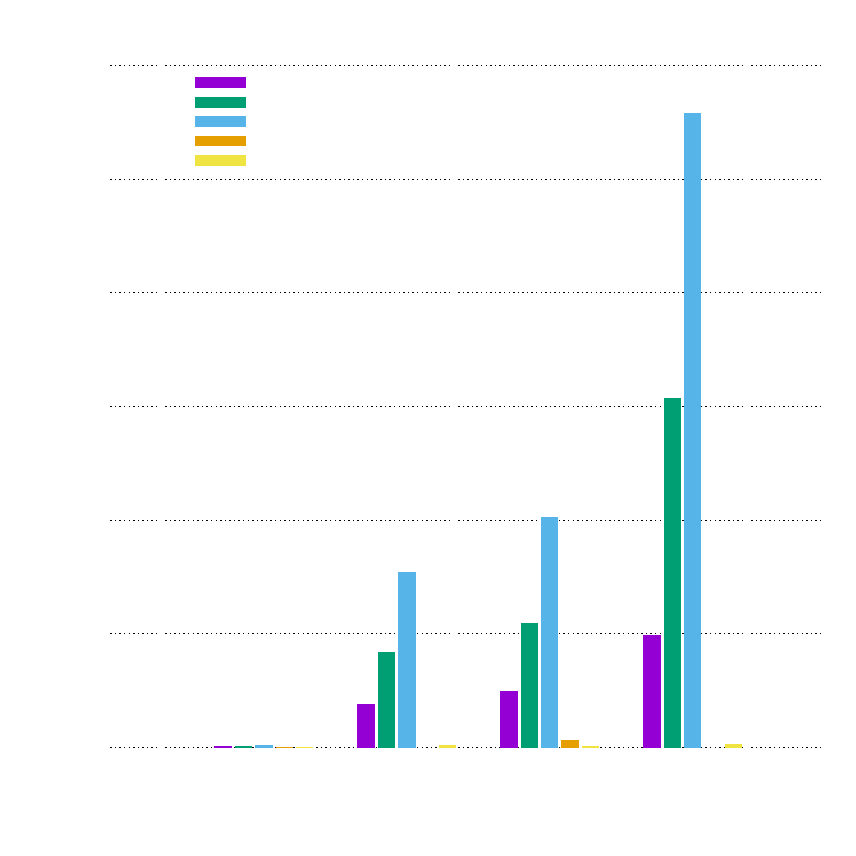
\includegraphics{desc_perf}}%
    \gplfronttext
  \end{picture}%
\endgroup

  \caption{Processing time for descriptors algorithms across the datasets. Similarly to figure~\ref{fig:plot:perf}, the data has been recorded during one run of the algorithm on Intel(R) Core(TM) i5-2520M and are intended to show order of magnitude differences of processing time between particular descriptors.}
  \label{fig:plot:desc_perf}
\end{figure}

\section{Initial estimate algorithm}

Comparing the presented reciprocal matching algorithm with \gls{SAC-IA}, the reciprocal matching algorithm produces better initial estimate in most of the evaluated cases (figure~\ref{fig:plot:desc_dist}). Significantly worse initial estimate was produced only for the \gls{FPFH} descriptors in ``Machine Hall'' dataset, which may not come as a surprise as the \gls{SAC-IA} algorithm was introduced with the \gls{FPFH} descriptors.

For \gls{PFH}, \gls{FPFH} and \gls{SHOT} descriptors the reciprocal matching algorithm produced better initial estimates in evaluation than the \gls{SAC-IA} algorithm. Especially for the \gls{PFH} and \gls{PFHRGB} descriptors the Euclidean error distance is significantly lower for the initial estimates produced by the reciprocal matching algorithm.
